\chapter{Differential Privacy Composition}

Among the 26 SIGMOD'26 papers tagged \texttt{privacy-dp}, composition accounting is close to a monoculture: 69\% of them assemble their end-to-end privacy guarantee by composing mechanisms, and the tool \texttt{dp-composition} is used by 18 of the 228 tagged papers overall, its strongest pairing being \texttt{privacy-guarantee} $\times$ \texttt{dp-composition} (16 papers). The arithmetic itself is shifting: the exemplars below still mostly add plain $(\epsilon,\delta)$ budgets, but the frontier results state composition for R\'enyi DP and $f$-DP, where the composed object is a whole divergence curve rather than a pair of scalars.

\section{The tool}

\begin{definition}[Differential privacy]
A randomized mechanism $\mathcal{M}:\mathcal{D}\to\mathcal{R}$ satisfies $(\epsilon,\delta)$-differential privacy if for all neighboring datasets $D\sim D'$ (differing in one record, edge, or node) and all measurable $S\subseteq\mathcal{R}$,
\[
\Pr[\mathcal{M}(D)\in S] \;\le\; e^{\epsilon}\cdot \Pr[\mathcal{M}(D')\in S] + \delta .
\]
With $\delta=0$ the guarantee is \emph{pure} $\epsilon$-DP \citep{dp-composition-bg1}.
\end{definition}

Five primitives, one line each:
\begin{itemize}
  \item \textbf{Sequential composition.} An adaptive sequence of releases with budgets $(\epsilon_i,\delta_i)$ satisfies $(\sum_i \epsilon_i,\ \sum_i \delta_i)$-DP: budgets add \citep{dp-composition-bg1,dp-composition-bg3}.
  \item \textbf{Post-processing immunity.} Any function of an $(\epsilon,\delta)$-DP output that does not touch the raw data is itself $(\epsilon,\delta)$-DP: analysis after the release is free \citep{dp-composition-bg3}.
  \item \textbf{Group privacy.} Datasets at distance $\lambda$ inherit $(\lambda\epsilon,\lambda\delta)$-DP: the guarantee degrades linearly in group size \citep{dp-composition-bg3}.
  \item \textbf{The R\'enyi ladder.} The Gaussian mechanism (noise $\mathcal{N}(0,\sigma^2 I)$, $\ell_2$-sensitivity $\Delta_2$) is $\bigl(\alpha,\ \alpha\Delta_2^2/(2\sigma^2)\bigr)$-RDP for every $\alpha>1$; RDP composes by adding the $\rho(\alpha)$; and $(\alpha,\rho)$-RDP converts to $\bigl(\rho(\alpha)+\log(1/\delta)/(\alpha-1),\ \delta\bigr)$-DP, optimized over $\alpha$ --- the engine behind $O(\epsilon\sqrt{k})$ rather than $k\epsilon$ for $k$ releases \citep{dp-composition-bg2,dp-composition-bg4}. $f$-DP makes the divergence curve itself the composed object \citep{dp-composition-bg5}.
  \item \textbf{Amplification by subsampling.} An $\epsilon$-DP mechanism run on a $p$-rate Poisson subsample satisfies $\log\!\bigl(1+p(e^{\epsilon}-1)\bigr)$-DP: smaller samples buy smaller budgets \citep{dp-composition-bg6}.
\end{itemize}

\section{Exemplars from SIGMOD'26}

\paragraph{Budget ledgers for private cluster explanations.}
The paper privately explains a given clustering by selecting the attribute combination that best accounts for it: top-$k$ candidate selection, then an exponential mechanism over combinations, then per-cluster histograms \cite{sigmod26-298}.

\begin{proposition}[Sequential composition]
Let $\mathcal{M}_1:\mathcal{D}\to\mathcal{R}_1$ and $\mathcal{M}_2:\mathcal{D}\times\mathcal{R}_1\to\mathcal{R}_2$. Suppose $\mathcal{M}_1$ satisfies $\epsilon_1$-DP and, for every $y\in\mathcal{R}_1$, $\mathcal{M}_2(\cdot,y)$ satisfies $\epsilon_2$-DP (as a function of its first input). Define $\mathcal{M}_3:\mathcal{D}\to\mathcal{R}_2$ by $\mathcal{M}_3(D)=\mathcal{M}_2(D,\mathcal{M}_1(D))$. Then $\mathcal{M}_3$ satisfies $(\epsilon_1+\epsilon_2)$-DP.
\end{proposition}

The end-to-end guarantee is the budget sum $\bigl(\epsilon_{\mathrm{CandSet}}+\epsilon_{\mathrm{TopComb}}+\epsilon_{\mathrm{Hist}}\bigr)$-DP, while inside the histogram stage the clusters are disjoint, so per-attribute and per-cluster releases compose \emph{in parallel}, each contributing $\epsilon_{\mathrm{Hist}}/2$ --- pure multiplicative $e^{\epsilon}$ arithmetic, no divergence needed.

\begin{center}
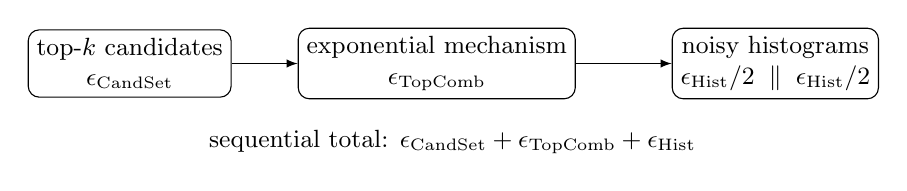
\begin{tikzpicture}[box/.style={draw,rounded corners,align=center,inner sep=3pt,font=\small}]
  \node[box] (a) at (0,0) {top-$k$ candidates\\ $\epsilon_{\mathrm{CandSet}}$};
  \node[box] (b) at (3.9,0) {exponential mechanism\\ $\epsilon_{\mathrm{TopComb}}$};
  \node[box] (c) at (8.2,0) {noisy histograms\\ $\epsilon_{\mathrm{Hist}}/2 \;\parallel\; \epsilon_{\mathrm{Hist}}/2$};
  \draw[-latex] (a) -- (b);
  \draw[-latex] (b) -- (c);
  \node[font=\small] at (4.1,-1.0) {sequential total: $\epsilon_{\mathrm{CandSet}}+\epsilon_{\mathrm{TopComb}}+\epsilon_{\mathrm{Hist}}$};
\end{tikzpicture}
\end{center}

\paragraph{Node-DP from edge-DP via group privacy.}
N2E converts any edge-DP graph mechanism into a node-DP one by clipping the input graph to a degree bound $\Delta^{*}$ that is itself privately approximated, then running the edge mechanism on the clipped graph \cite{sigmod26-337}.

\begin{lemma}[Group privacy]
If a mechanism $\mathcal{M}$ satisfies $(\epsilon,\delta)$-differential privacy, then for any two graphs $G,G'$ with $d(G,G')=\lambda$ (i.e., differing by $\lambda$ edges or nodes) and any subset of outputs $S\subseteq\mathcal{R}$,
\[
\Pr[\mathcal{M}(G)\in S] \;\le\; e^{\lambda\epsilon}\cdot \Pr[\mathcal{M}(G')\in S] + \lambda\delta .
\]
The mechanism satisfies $(\lambda\epsilon,\lambda\delta)$-DP for the group of $\lambda$ edges or nodes.
\end{lemma}

The composition primitive doing the lifting is group privacy: a one-node change is a group of $\lambda$ edge changes, so the edge-DP calculus transfers to node-DP neighborhoods. The degree search spends sparse-vector-technique queries at a logarithmic scale, so only logarithmically many sequential compositions are consumed before post-processing turns the noisy degree into the clipping $\Delta^{*}$; the whole framework satisfies $(\epsilon,\delta)$-node-DP \cite{sigmod26-337}.

\paragraph{Per-record budgets: composition of functions, not scalars.}
Per-record DP replaces the global $\epsilon$ by a budget function $\epsilon_{\mathcal{E}}(r)$ (a bank may assign wealthier clients smaller budgets), and estimates sums/counts by partitioning records into geometrically doubling budget slices, one Laplace mechanism per slice \cite{sigmod26-263}.

\begin{lemma}[PrDP parallel composition]
Let $R_1,\dots,R_k$ be disjoint subdomains and $\mathcal{M}_1,\dots,\mathcal{M}_k$ a series of $\mathcal{E}_i$-PrDP mechanisms. Their parallel composition $\mathcal{M}(D):=\bigl(\mathcal{M}_1(D_{R_1}),\dots,\mathcal{M}_k(D_{R_k})\bigr)$ satisfies $\mathcal{E}'$-PrDP, where $\mathcal{E}'(r)=\max\{\mathcal{E}_i(r)\}_{i=1}^{k}$ for all $r\in[U]^d$.
\end{lemma}

Here the composed object is a budget \emph{function}: releases on disjoint subdomains take a pointwise maximum instead of a sum, so a record is only ever charged the largest budget of any slice touching it. Near-optimality of the resulting error is certified against down-neighborhood lower bounds \cite{sigmod26-263}.

\paragraph{Concurrent composition for continual mechanisms.}
Continual mechanisms answer streams of queries; the hard question is what composition survives an adversary who adaptively and \emph{concurrently} interleaves access to many such mechanisms \cite{sigmod26-049}.

\begin{theorem}[Concurrent composition of continual mechanisms, informal]
The concurrent composition of continual mechanisms $\mathcal{M}_i$ that are $(\epsilon_i,\delta_i)$-DP with respect to a verification function $f_i$ is $(\epsilon,\delta)$-DP for the same $(\epsilon,\delta)$ that holds for composing noninteractive mechanisms that are $(\epsilon_i,\delta_i)$-DP. This allows the adversary to adaptively and concurrently choose the neighboring sequences fed to each $\mathcal{M}_i$ based on the responses received from the other mechanisms.
\end{theorem}

What carries the guarantee is a simulation: every $(\epsilon,\delta)$-DP interactive mechanism can be realized by interactive post-processing of randomized-response outputs, so the divergence arithmetic of ordinary composition transfers verbatim to concurrent adversaries. The same paper pushes the frontier from $(\epsilon,\delta)$ to $f$-DP and R\'enyi DP, complete with a counterexample showing where intuition breaks --- the direction in which the currency is moving. \cite{sigmod26-049}\pods

\paragraph{Composing obliviousness in a multi-way join.}
The differentially oblivious join evaluates queries in untrusted memory while leaking only the input size $|I|$ plus a DP-noisy upper bound $\widehat{OUT}$ on the join size \cite{sigmod26-073}.

\begin{theorem}[Meta-join]
Algorithm~1 is $(\epsilon_1+\epsilon_2,\ \delta_1+\delta_2)$-DO.
\end{theorem}

Two primitives carry it: an $(\epsilon_1,\delta_1)$-DO subroutine releases the $(\epsilon_2,\delta_2)$-DP bound $\widehat{OUT}$, and the advised join's access pattern is a deterministic function of $|I|$ and $\widehat{OUT}$ only. Sequential composition adds both coordinates, and post-processing immunity is precisely what makes an \emph{access pattern} a legitimate object to compose \cite{sigmod26-073}.

\begin{reachbox}{When to reach for DP composition}
Reach for it whenever a system releases \emph{several} interacting statistics and the privacy proof is a ledger: candidate selections, noisy summaries, clipped releases. Then budgets add (exemplars 1 and 5 above, with $\delta$'s summed too in the approximate case), disjoint data slices switch the arithmetic from sums to maxima (exemplars 1 and 3), and group privacy reduces an expensive neighborhood (node-DP) to a cheap one (edge-DP) at linear cost in group size (exemplar 2). Reach for divergence arithmetic --- RDP or $f$-DP curves --- when many releases would make summed $\epsilon$'s vacuous, buying $O(\epsilon\sqrt{k})$ over $k\epsilon$ (the frontier of exemplar 4); reach for subsampling amplification when releases are computed on samples anyway. Post-processing immunity ships every downstream artifact --- clipped graphs, access patterns, indices --- for free. Skip the machinery when a single calibrated release suffices, or when every output is a post-processing of one DP output: composing there only overcounts.
\end{reachbox}
